\documentclass[11pt,a4paper]{article}

\usepackage[utf8]{inputenc}
\usepackage[T1]{fontenc}
\usepackage[spanish,es-nodecimaldot]{babel}
\usepackage{lmodern}
\usepackage{amsmath}
\usepackage{amssymb}
\usepackage{booktabs}
\usepackage{array}
\usepackage{float}
\usepackage{geometry}
\usepackage{graphicx}
\usepackage{subcaption}
\usepackage{placeins}
\usepackage{hyperref}

\geometry{margin=2.5cm}
\graphicspath{{../plots/}}
\addto\captionsspanish{\renewcommand{\tablename}{Tabla}}

\hypersetup{
    colorlinks=true,
    linkcolor=black,
    urlcolor=blue
}

\newcommand{\pendiente}[1]{%
    \par\smallskip
    \noindent\fbox{%
        \begin{minipage}{0.94\linewidth}
        \textbf{Pendiente para completar:} #1
        \end{minipage}%
    }
    \par\smallskip
}

\title{Trabajo Práctico Nro. 2\\Control de Rumbo y Reconstrucción de Trayectoria de una Embarcación}
\author{Nombres completos del grupo}
\date{IOR442 Sistemas de Control}

\begin{document}

\maketitle
\tableofcontents
\newpage

\section{Introducción}

En este trabajo se estudia el control de rumbo de una embarcación navegando con velocidad longitudinal constante $u_0 = 2\,\mathrm{m/s}$. El sistema de control considerado es SISO: la entrada es el momento de control en yaw $\tau_r$ y la salida controlada es el ángulo de rumbo $\psi$.

El informe sigue la estructura de la consigna: primero se diseña un controlador por asignación de polos con acción integral, luego se reconstruye la trayectoria en el plano inercial y finalmente se compara el desempeño contra distintos diseños LQI.

\pendiente{Completar nombres del grupo y, si se desea, agregar una breve descripción del criterio general usado para comparar los controladores.}

\section{Versiones y dependencias}

El código fue ejecutado con las versiones indicadas en la Tabla~\ref{tab:versiones}. Las dependencias también se listan en el archivo \texttt{requirements.txt}.

\begin{table}[H]
\centering
\caption{Versiones utilizadas para ejecutar los notebooks y generar los resultados.}
\label{tab:versiones}
\begin{tabular}{ll}
\toprule
Componente & Versión \\
\midrule
Python & 3.11.15 \\
NumPy & 2.4.4 \\
SciPy & 1.17.1 \\
Matplotlib & 3.10.8 \\
python-control & 0.10.2 \\
Pandas & 2.3.3 \\
Jupyter Notebook & 7.5.5 \\
\bottomrule
\end{tabular}
\end{table}


\section{Parte A - Control de rumbo con asignación de polos}

\subsection{Modelo en espacio de estados}

Con el vector de estados $x = [v\ r\ \psi]^T$, la entrada $u_c = \tau_r$ y la salida $y = \psi$, el modelo lineal puede escribirse como

\begin{equation}
\dot{x} = A x + B u_c, \qquad y = Cx + Du_c,
\end{equation}

donde

\begin{equation}
A =
\begin{bmatrix}
-0.25 & -2 & 0 \\
0.08 & -0.35 & 0 \\
0 & 1 & 0
\end{bmatrix},
\quad
B =
\begin{bmatrix}
0 \\
0.62 \\
0
\end{bmatrix},
\quad
C =
\begin{bmatrix}
0 & 0 & 1
\end{bmatrix},
\quad
D = 0.
\end{equation}

\subsection{Controlabilidad del sistema original}

La matriz de controlabilidad del sistema original se define como

\begin{equation}
\mathcal{C} =
\begin{bmatrix}
B & AB & A^2B
\end{bmatrix}
=
\begin{bmatrix}
0 & -1.2400 & 0.7440 \\
0.6200 & -0.2170 & -0.0233 \\
0 & 0.6200 & -0.2170
\end{bmatrix}.
\label{eq:controlabilidad-original}
\end{equation}

Como $\operatorname{rango}(\mathcal{C})=3$, la matriz tiene rango completo e igual a la dimensión del sistema original. Por lo tanto, es posible diseñar un controlador por realimentación completa de estados para el modelo de rumbo.

\subsection{Sistema aumentado con acción integral}

Para eliminar el error estacionario frente a referencias constantes o por tramos se incorpora el estado integral

\begin{equation}
\dot{\xi} = \psi_{ref} - \psi.
\end{equation}

El vector aumentado es $x_a = [v\ r\ \psi\ \xi]^T$ y el sistema queda

\begin{equation}
\dot{x}_a = A_a x_a + B_a \tau_r + E_a \psi_{ref},
\end{equation}

con

\begin{equation}
A_a =
\begin{bmatrix}
-0.25 & -2 & 0 & 0 \\
0.08 & -0.35 & 0 & 0 \\
0 & 1 & 0 & 0 \\
0 & 0 & -1 & 0
\end{bmatrix},
\quad
B_a =
\begin{bmatrix}
0 \\
0.62 \\
0 \\
0
\end{bmatrix},
\quad
E_a =
\begin{bmatrix}
0 \\
0 \\
0 \\
1
\end{bmatrix}.
\end{equation}

\subsection{Controlabilidad del sistema aumentado}

La matriz de controlabilidad del sistema aumentado es

\begin{equation}
\mathcal{C}_a =
\begin{bmatrix}
B_a & A_aB_a & A_a^2B_a & A_a^3B_a
\end{bmatrix}
=
\begin{bmatrix}
0 & -1.2400 & 0.7440 & -0.1395 \\
0.6200 & -0.2170 & -0.0233 & 0.0677 \\
0 & 0.6200 & -0.2170 & -0.0233 \\
0 & 0 & -0.6200 & 0.2170
\end{bmatrix}.
\label{eq:controlabilidad-aumentado}
\end{equation}

Como $\operatorname{rango}(\mathcal{C}_a)=4$, la matriz tiene rango completo e igual a la dimensión del sistema aumentado. Por lo tanto, es posible asignar arbitrariamente los polos del sistema aumentado.

\subsection{Diseño del controlador}

Se utiliza la ley de control

\begin{equation}
\tau_r = -K_a x_a = -K_x x - k_i \xi,
\qquad
K_a = [k_v\ k_r\ k_\psi\ k_i].
\end{equation}

Primero se eligieron los polos deseados del sistema aumentado y luego se calculó la ganancia $K_a$. Para ello se utilizó la función \texttt{control.place}. Esta función es un wrapper de \texttt{scipy.signal.place\_poles}, que implementa el algoritmo de Tits-Yang para asignación robusta de polos por realimentación de estados.

Los polos asignados y la ganancia obtenida se muestran, en ese orden, en las Tablas~\ref{tab:parte-a-polos} y~\ref{tab:parte-a-ganancias}.

\begin{table}[H]
\centering
\caption{Polos asignados para el sistema aumentado de la Parte A.}
\label{tab:parte-a-polos}
\begin{tabular}{cccc}
\toprule
$p_1$ & $p_2$ & $p_3$ & $p_4$ \\
\midrule
-1.500 & -2.000 & -2.500 & -3.000 \\
\bottomrule
\end{tabular}
\end{table}

\begin{table}[H]
\centering
\caption{Ganancia del controlador por asignación de polos de la Parte A.}
\label{tab:parte-a-ganancias}
\begin{tabular}{rrrr}
\toprule
$k_v$ & $k_r$ & $k_\psi$ & $k_i$ \\
\midrule
-174.518 & 13.548 & -304.839 & -145.161 \\
\bottomrule
\end{tabular}
\end{table}


\subsection{Simulación de seguimiento}

La simulación se realiza durante $T_f = 60\,\mathrm{s}$ utilizando la referencia por tramos pedida en la consigna. En la Figura~\ref{fig:parte-a-seguimiento} se muestra el seguimiento de rumbo.

\begin{figure}[H]
\centering
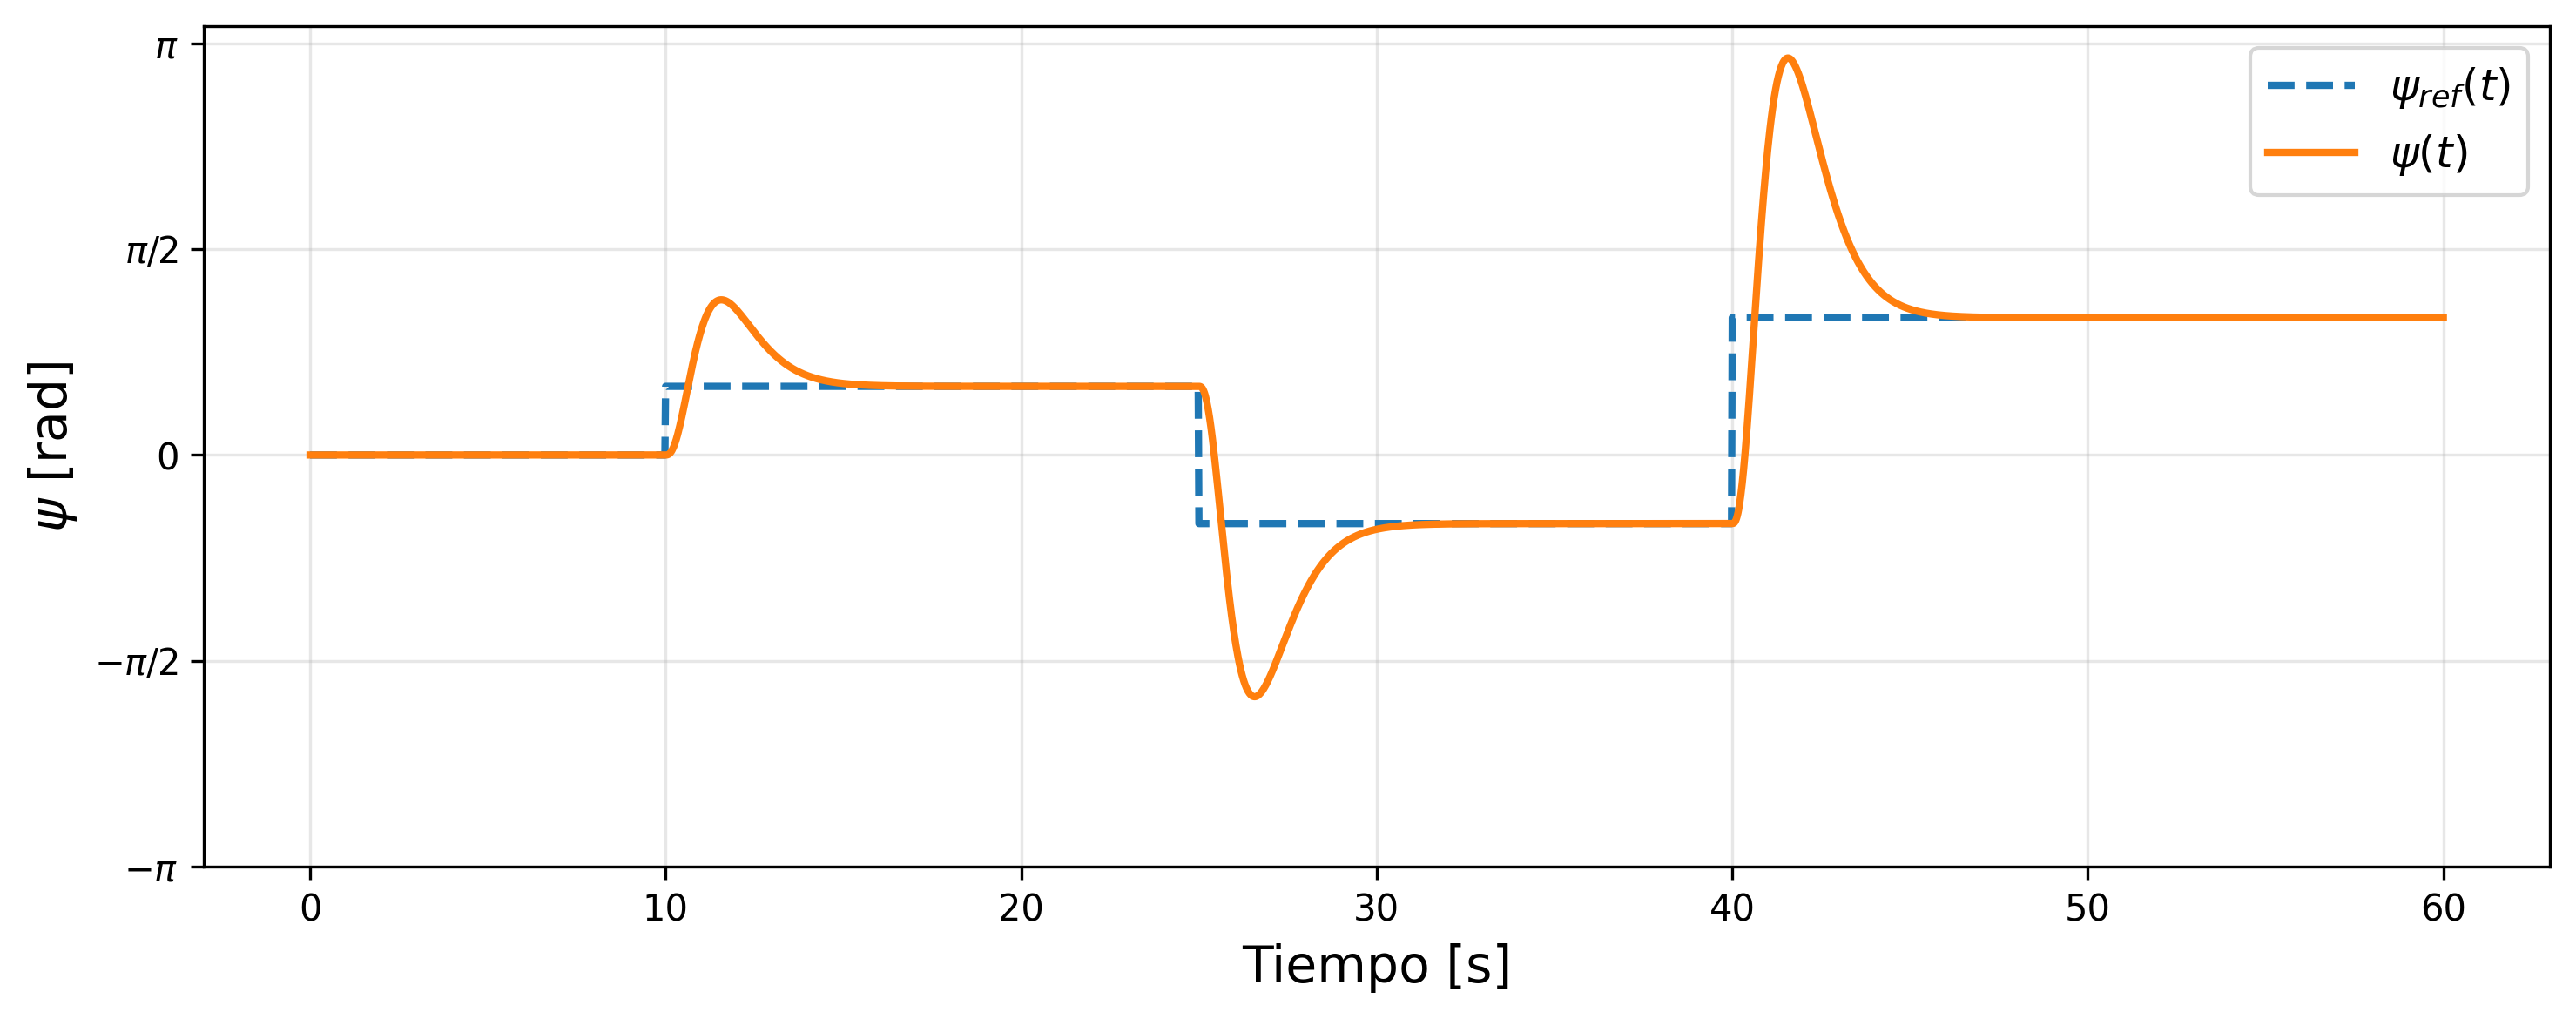
\includegraphics[width=0.86\textwidth]{parteA/seguimiento.png}
\caption{Seguimiento de referencia de rumbo para el controlador por asignación de polos.}
\label{fig:parte-a-seguimiento}
\end{figure}

\subsection{Error, estados y señal de control}

La Figura~\ref{fig:parte-a-error-estados-control} resume el error de seguimiento, los estados del sistema y la señal de control. Las métricas principales se muestran en la Tabla~\ref{tab:parte-a-metricas}.

\begin{figure}[H]
\centering
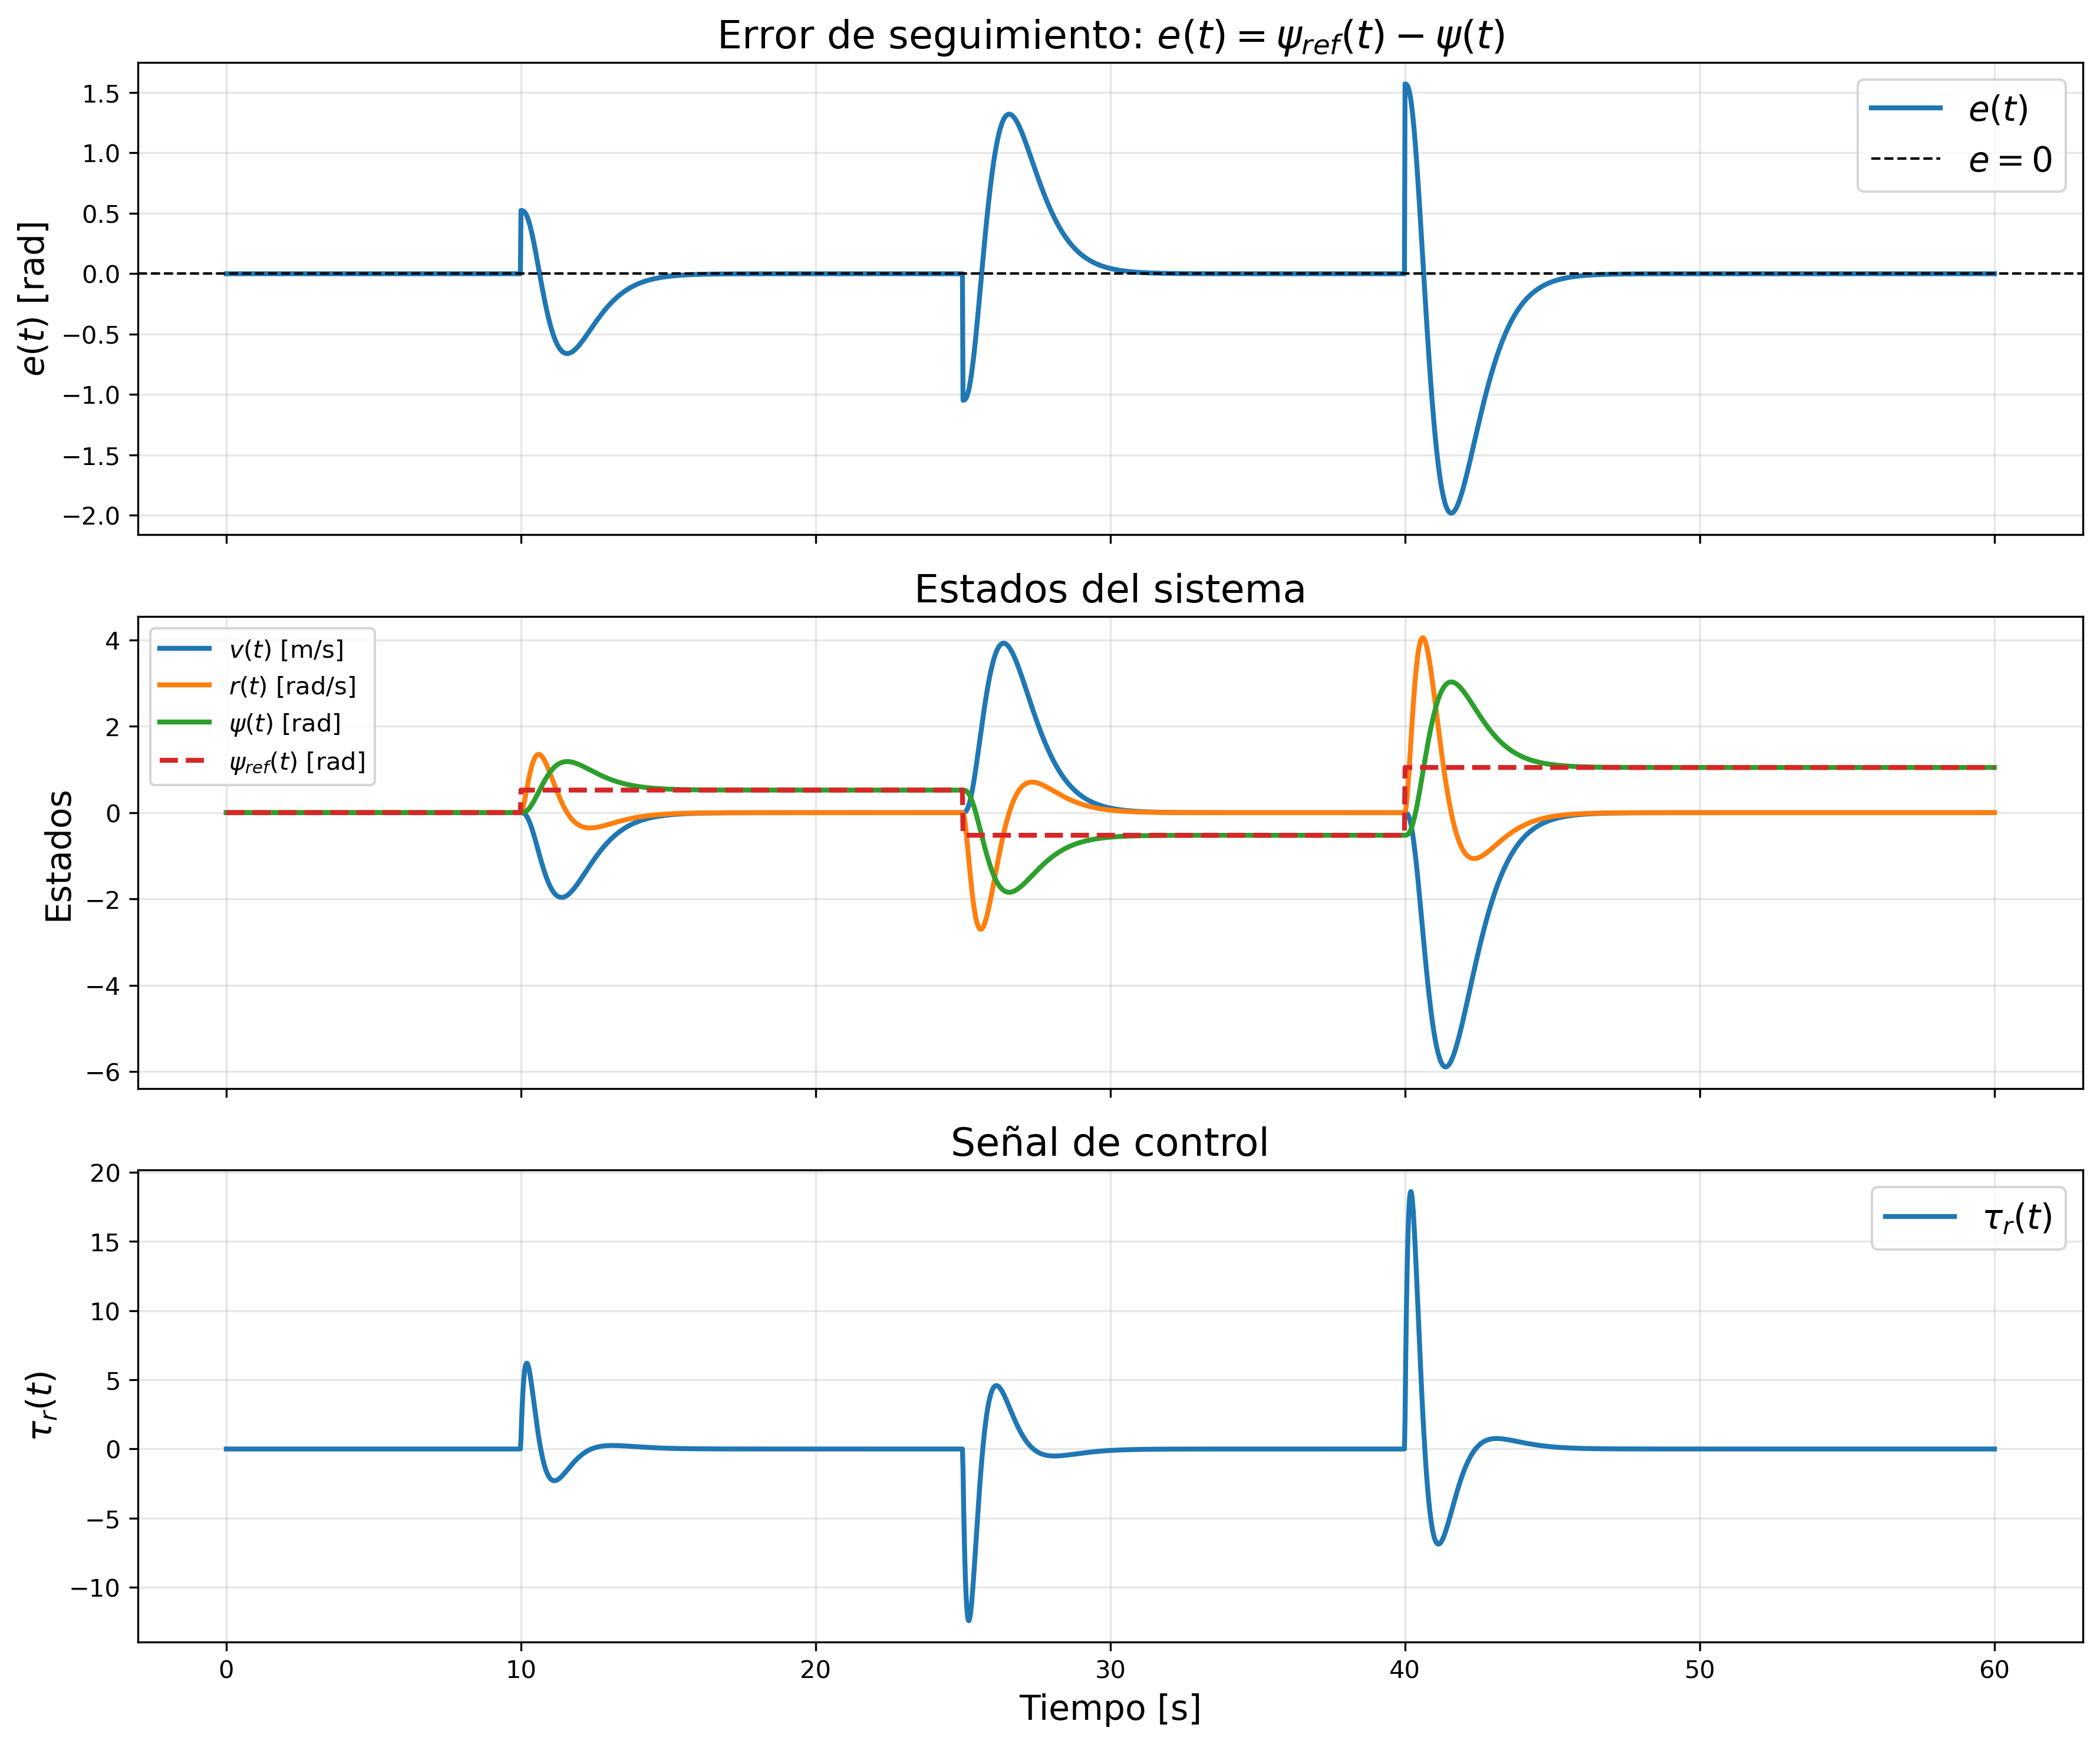
\includegraphics[width=0.92\textwidth]{parteA/error_estados_control.png}
\caption{Error de seguimiento, estados y señal de control para la Parte A.}
\label{fig:parte-a-error-estados-control}
\end{figure}

\begin{table}[H]
\centering
\caption{Métricas principales de la simulación de la Parte A.}
\label{tab:parte-a-metricas}
\begin{tabular}{lr}
\toprule
Métrica & Valor \\
\midrule
$\max |e(t)|$ & 1.9810 \\
$e(T_f)$ & 0.0000 \\
IAE & 9.2710 \\
ISE & 9.8294 \\
$\max |\tau_r(t)|$ & 18.5989 \\
RMS de $\tau_r(t)$ & 1.9077 \\
$\max |v(t)|$ & 5.8903 \\
$\max |r(t)|$ & 4.0537 \\
$\max |\psi(t)|$ & 3.0282 \\
\bottomrule
\end{tabular}
\end{table}


\subsection{Discusión de desempeño}

\pendiente{Discutir si la embarcación sigue la referencia, si el error estacionario es nulo, si la velocidad de respuesta es adecuada, la suavidad de $\tau_r$, los valores máximos requeridos de $\tau_r$, el efecto esperado al mover los polos y las limitaciones físicas del actuador.}

\FloatBarrier

\section{Parte B - Reconstrucción de trayectoria en el plano}

\subsection{Ecuaciones cinemáticas}

La velocidad en el sistema del cuerpo se escribe como $[u_0\ v]^T$. Para expresarla en el sistema inercial se aplica una rotación de ángulo $\psi$:

\begin{equation}
\begin{bmatrix}
\dot{X} \\
\dot{Y}
\end{bmatrix}
=
\begin{bmatrix}
\cos\psi & -\sin\psi \\
\sin\psi & \cos\psi
\end{bmatrix}
\begin{bmatrix}
u_0 \\
v
\end{bmatrix}.
\end{equation}

De esta forma se obtiene

\begin{equation}
\dot{X} = u_0 \cos(\psi) - v \sin(\psi),
\qquad
\dot{Y} = u_0 \sin(\psi) + v \cos(\psi).
\end{equation}

\subsection{Integración de la trayectoria}

La trayectoria se reconstruye a partir de las señales $v(t)$ y $\psi(t)$ obtenidas en la Parte A, con $X(0)=0$ e $Y(0)=0$. La integración numérica se realiza con la misma grilla temporal de simulación.

\begin{table}[H]
\centering
\caption{Condición inicial y posición final reconstruida en la Parte B.}
\label{tab:parte-b-posicion}
\begin{tabular}{lrr}
\toprule
Caso & $X$ [m] & $Y$ [m] \\
\midrule
Inicial & 0.00 & 0.00 \\
Final Parte B & 97.40 & 38.14 \\
\bottomrule
\end{tabular}
\end{table}


\subsection{Trayectoria obtenida}

La Figura~\ref{fig:parte-b-trayectoria} muestra la trayectoria reconstruida en el plano inercial.

\begin{figure}[H]
\centering
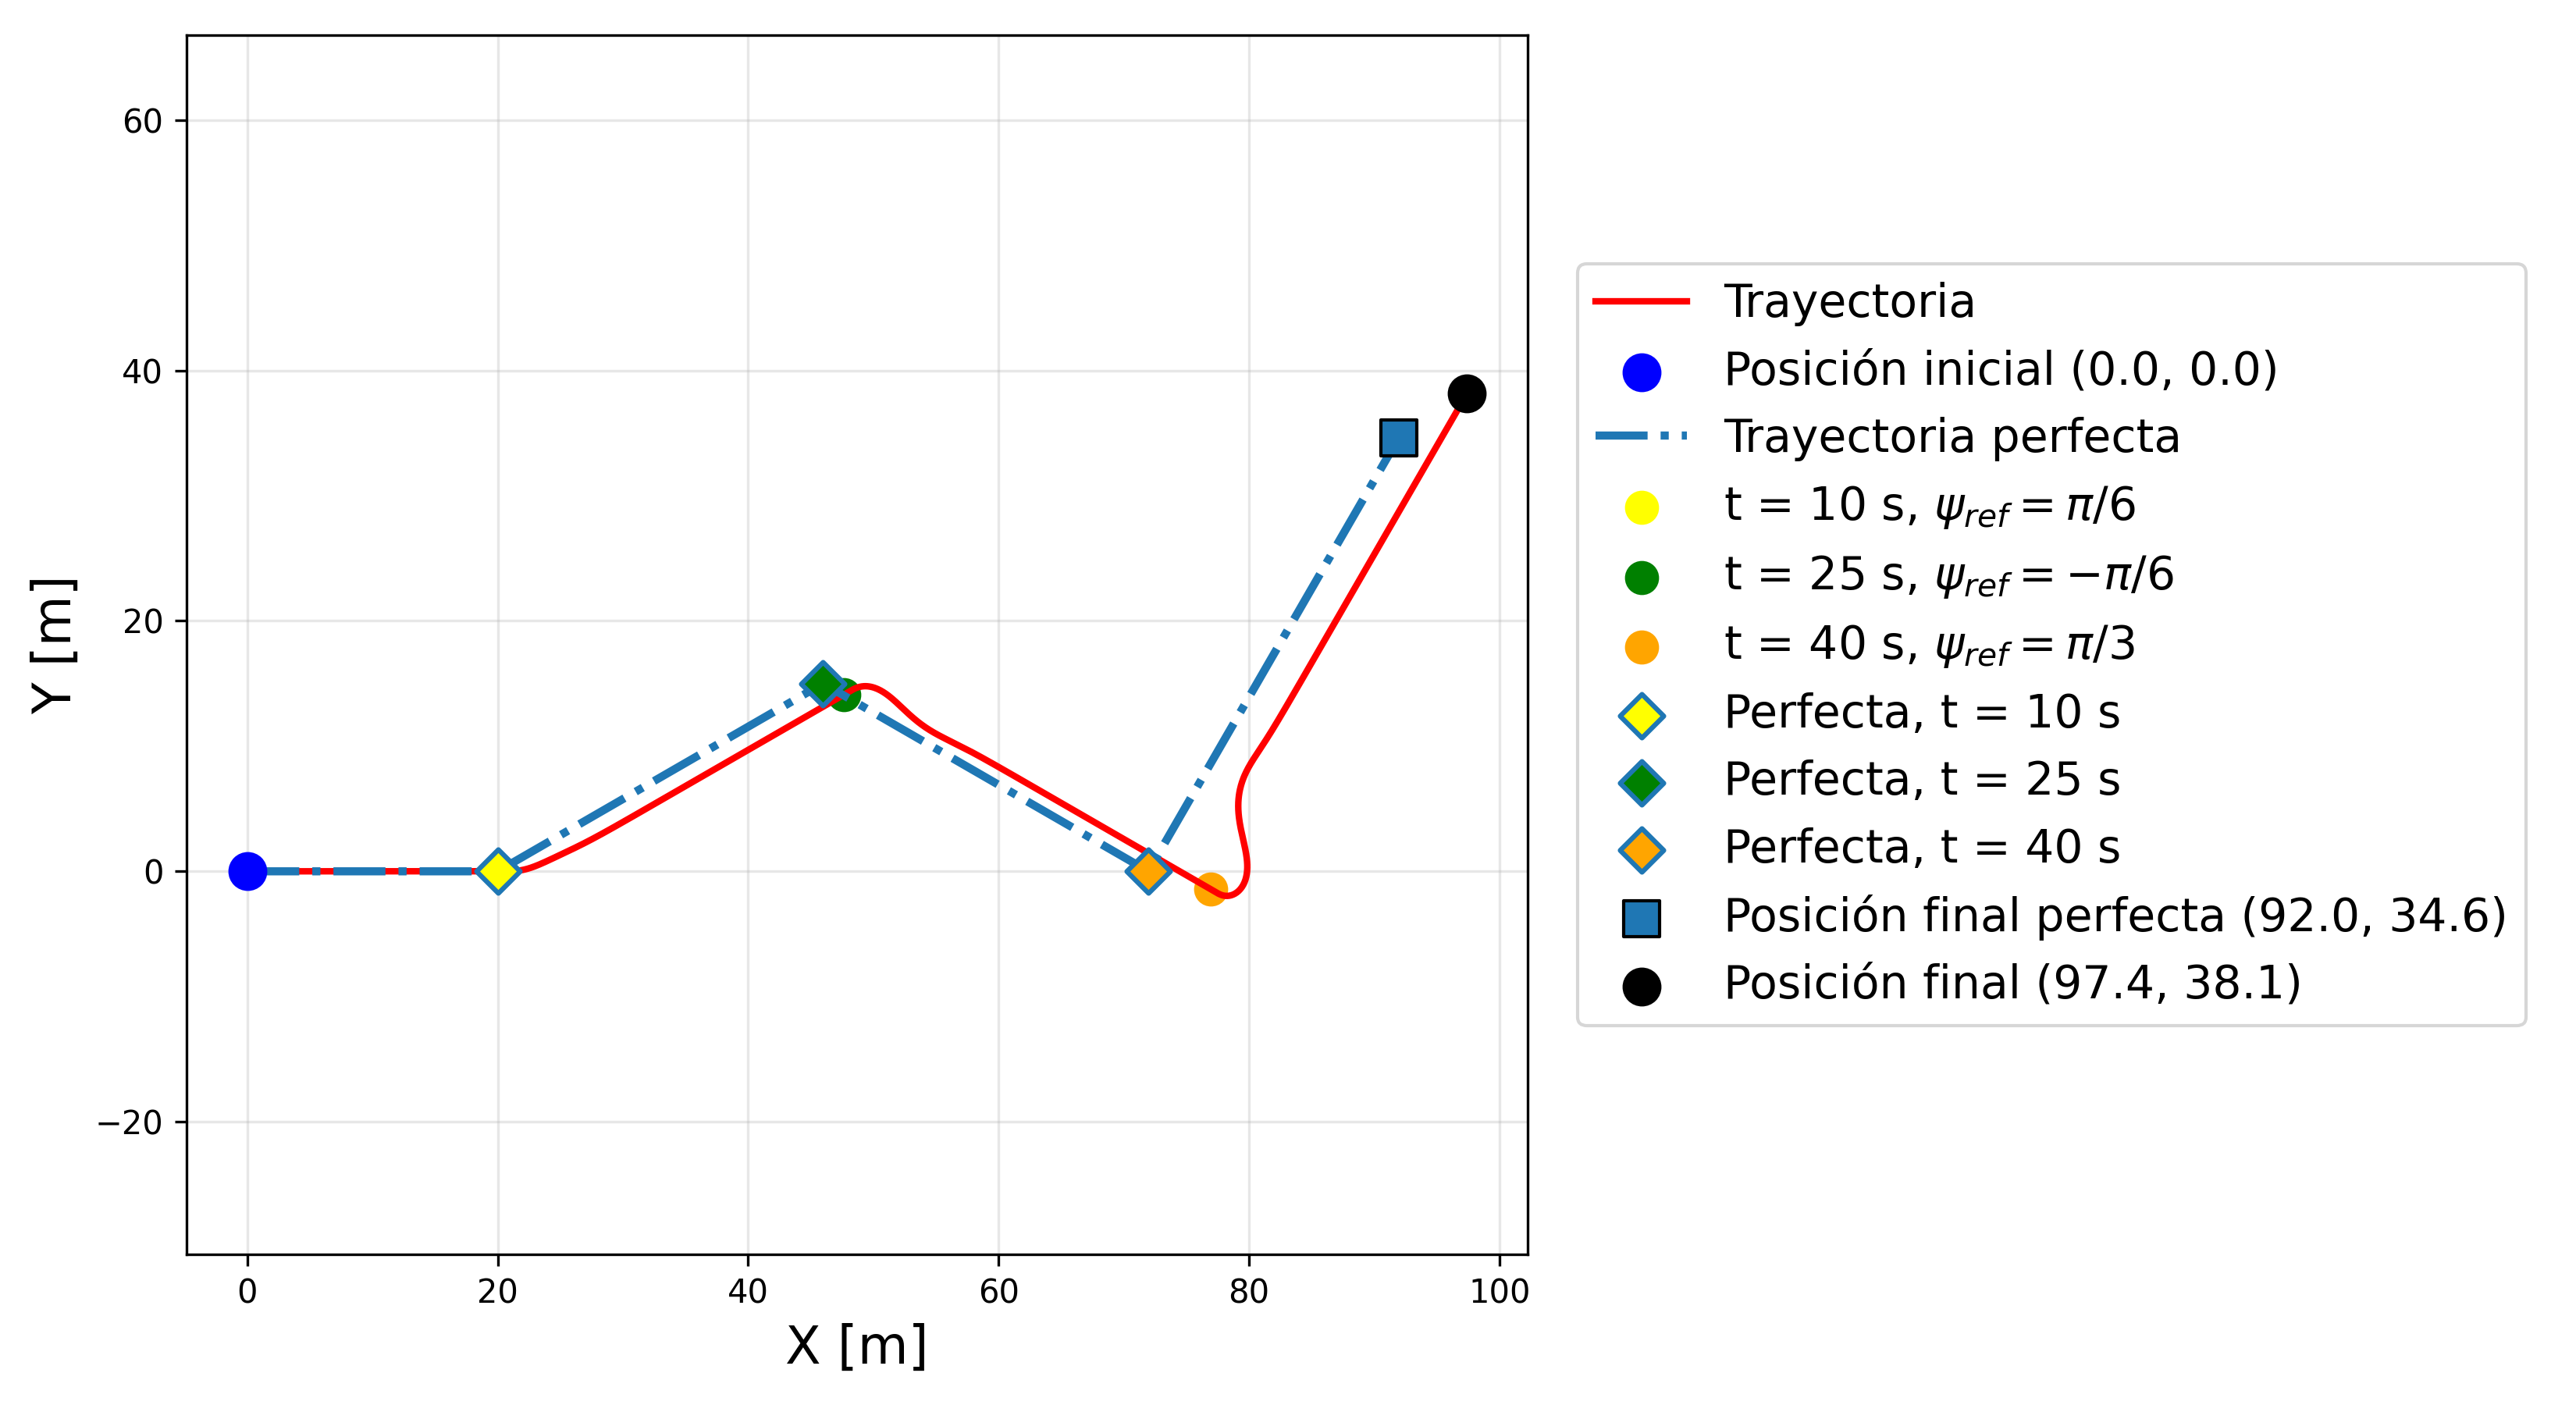
\includegraphics[width=0.82\textwidth]{parteB/trayectoria.png}
\caption{Trayectoria reconstruida con el controlador de la Parte A.}
\label{fig:parte-b-trayectoria}
\end{figure}

\subsection{Análisis de la trayectoria}

Se observa en la figura~\ref{fig:parte-b-trayectoria} que en cada cambio de trayectoria, el controlador logra orientar la embarcación correctamente. Sin embargo, como no es posible hacer el ajuste de forma instantánea, la trayectoria real acumula un pequeño error contra la trayectoria perfecta en cada giro. Este comportamiento se puede observar principalmente en el instante $t=40\,s$.

Como se vio en la parte A, con polos situados más a la izquiera se podrían conseguir respuestas más rápidas y reducir el error, a costo de picos altos en la señal de control y cambios más bruscos.

Incluso con un control más fuerte, según las ecuaciones cinemáticas, $v(t)$ afecta a $\dot{X}$ e $\dot{Y}$ con $-v\sin(\psi)$ y $+v\cos(\psi)$, respectivamente. Esto significa que incluso si el ángulo de rumbo $\psi$ fuera exactamente el deseado, la presencia de $v(t)$ hace que la dirección real de desplazamiento difiera levemente de la dirección apuntada por el barco.

\subsection{Discusión}
Si se quisiera controlar directamente la posición en el plano $XY$, sería necesario reformular el problema incorporando realimentación de posición y pasando a MIMO. 
Esto no se podría resolver con el controlador diseñado en la Parte A, ya que la relación entre la entrada de control ($\tau_r$) y las posiciones $X$, $Y$ en el plano es no lineal porque que depende de $\sin(\psi)$ y $\cos(\psi)$.
Para controlar la posición, se tendría que diseñar un controlador no lineal o linealizar el sistema alrededor de un punto para luego aplicar técnicas de control lineal.

\FloatBarrier

\section{Parte C - Control de rumbo mediante LQI}

\subsection{Ecuación de estado y función de costo}

Se utiliza el mismo sistema aumentado de la Parte A:

\begin{equation}
\dot{x}_a = A_a x_a + B_a \tau_r + E_a \psi_{ref}.
\end{equation}

El controlador LQI se obtiene minimizando una función de costo cuadrática de la forma

\begin{equation}
J = \int_0^\infty \left(x_a^T Q_a x_a + \tau_r^T R \tau_r\right) dt.
\end{equation}

La matriz $Q_a$ pondera los estados aumentados $v$, $r$, $\psi$ y $\xi$, mientras que $R$ pondera el esfuerzo de control.

\subsection{Aplicabilidad del LQI}

El sistema aumentado es controlable, como se verificó mediante la matriz de controlabilidad de la Ecuación~\eqref{eq:controlabilidad-aumentado} en la Parte A. Por lo tanto, es posible aplicar un diseño LQI sobre el modelo aumentado con integrador.

\subsection{Matrices de ponderación evaluadas}

La Tabla~\ref{tab:parte-c-ponderaciones} resume los seis casos evaluados. Se incluyeron variantes agresivas, intermedias, penalizadas en velocidad lateral y de menor esfuerzo de control.

\begin{table}[H]
\centering
\caption{Matrices de ponderación evaluadas para el diseño LQI. Se muestra la diagonal de $Q_a$.}
\label{tab:parte-c-ponderaciones}
\small
\begin{tabular}{lrrrrr}
\toprule
Caso & $q_v$ & $q_r$ & $q_\psi$ & $q_\xi$ & $R$ \\
\midrule
MUY\_AGRESIVO & 1 & 1 & 80 & 150 & 0.5 \\
AGRESIVO & 1 & 1 & 50 & 100 & 1 \\
INTERMEDIO & 1 & 2 & 30 & 80 & 10 \\
V\_PENALIZADO & 10 & 5 & 30 & 80 & 10 \\
SUAVE & 1 & 5 & 20 & 50 & 50 \\
CONTROL\_ECONOMICO & 1 & 5 & 10 & 20 & 200 \\
\bottomrule
\end{tabular}
\end{table}


\subsection{Ganancias, polos y simulaciones}

Las ganancias y polos resultantes se muestran en las Tablas~\ref{tab:parte-c-ganancias} y~\ref{tab:parte-c-polos}. La Figura~\ref{fig:parte-c-polos} muestra la ubicación de polos en el plano complejo.

\begin{table}[H]
\centering
\caption{Ganancias obtenidas para cada controlador LQI.}
\label{tab:parte-c-ganancias}
\small
\begin{tabular}{lrrrr}
\toprule
Caso & $k_v$ & $k_r$ & $k_\psi$ & $k_i$ \\
\midrule
MUY\_AGRESIVO & 0.107 & 7.838 & 21.382 & -17.321 \\
AGRESIVO & 0.110 & 6.120 & 13.665 & -10.000 \\
INTERMEDIO & 0.121 & 3.466 & 5.117 & -2.828 \\
V\_PENALIZADO & 0.071 & 3.667 & 5.438 & -2.828 \\
SUAVE & 0.120 & 2.190 & 2.461 & -1.000 \\
CONTROL\_ECONOMICO & 0.111 & 1.248 & 1.134 & -0.316 \\
\bottomrule
\end{tabular}
\end{table}

\begin{table}[H]
\centering
\caption{Polos de lazo cerrado obtenidos para cada controlador LQI.}
\label{tab:parte-c-polos}
\small
\setlength{\tabcolsep}{4pt}
\begin{tabular}{lccc}
\toprule
Caso & Par complejo & Polo real 1 & Polo real 2 \\
\midrule
MUY\_AGRESIVO & $-1.948 \pm 2.091i$ & $-1.314$ & $-0.250$ \\
AGRESIVO & $-1.430 \pm 1.666i$ & $-1.284$ & $-0.250$ \\
INTERMEDIO & $-0.722 \pm 1.067i$ & $-0.251$ & $-1.055$ \\
V\_PENALIZADO & $-0.849 \pm 1.072i$ & $-0.922$ & $-0.254$ \\
SUAVE & $-0.477 \pm 0.768i$ & $-0.252$ & $-0.752$ \\
CONTROL\_ECONOMICO & $-0.336 \pm 0.552i$ & $-0.275$ & $-0.427$ \\
\bottomrule
\end{tabular}
\end{table}


\begin{figure}[H]
\centering
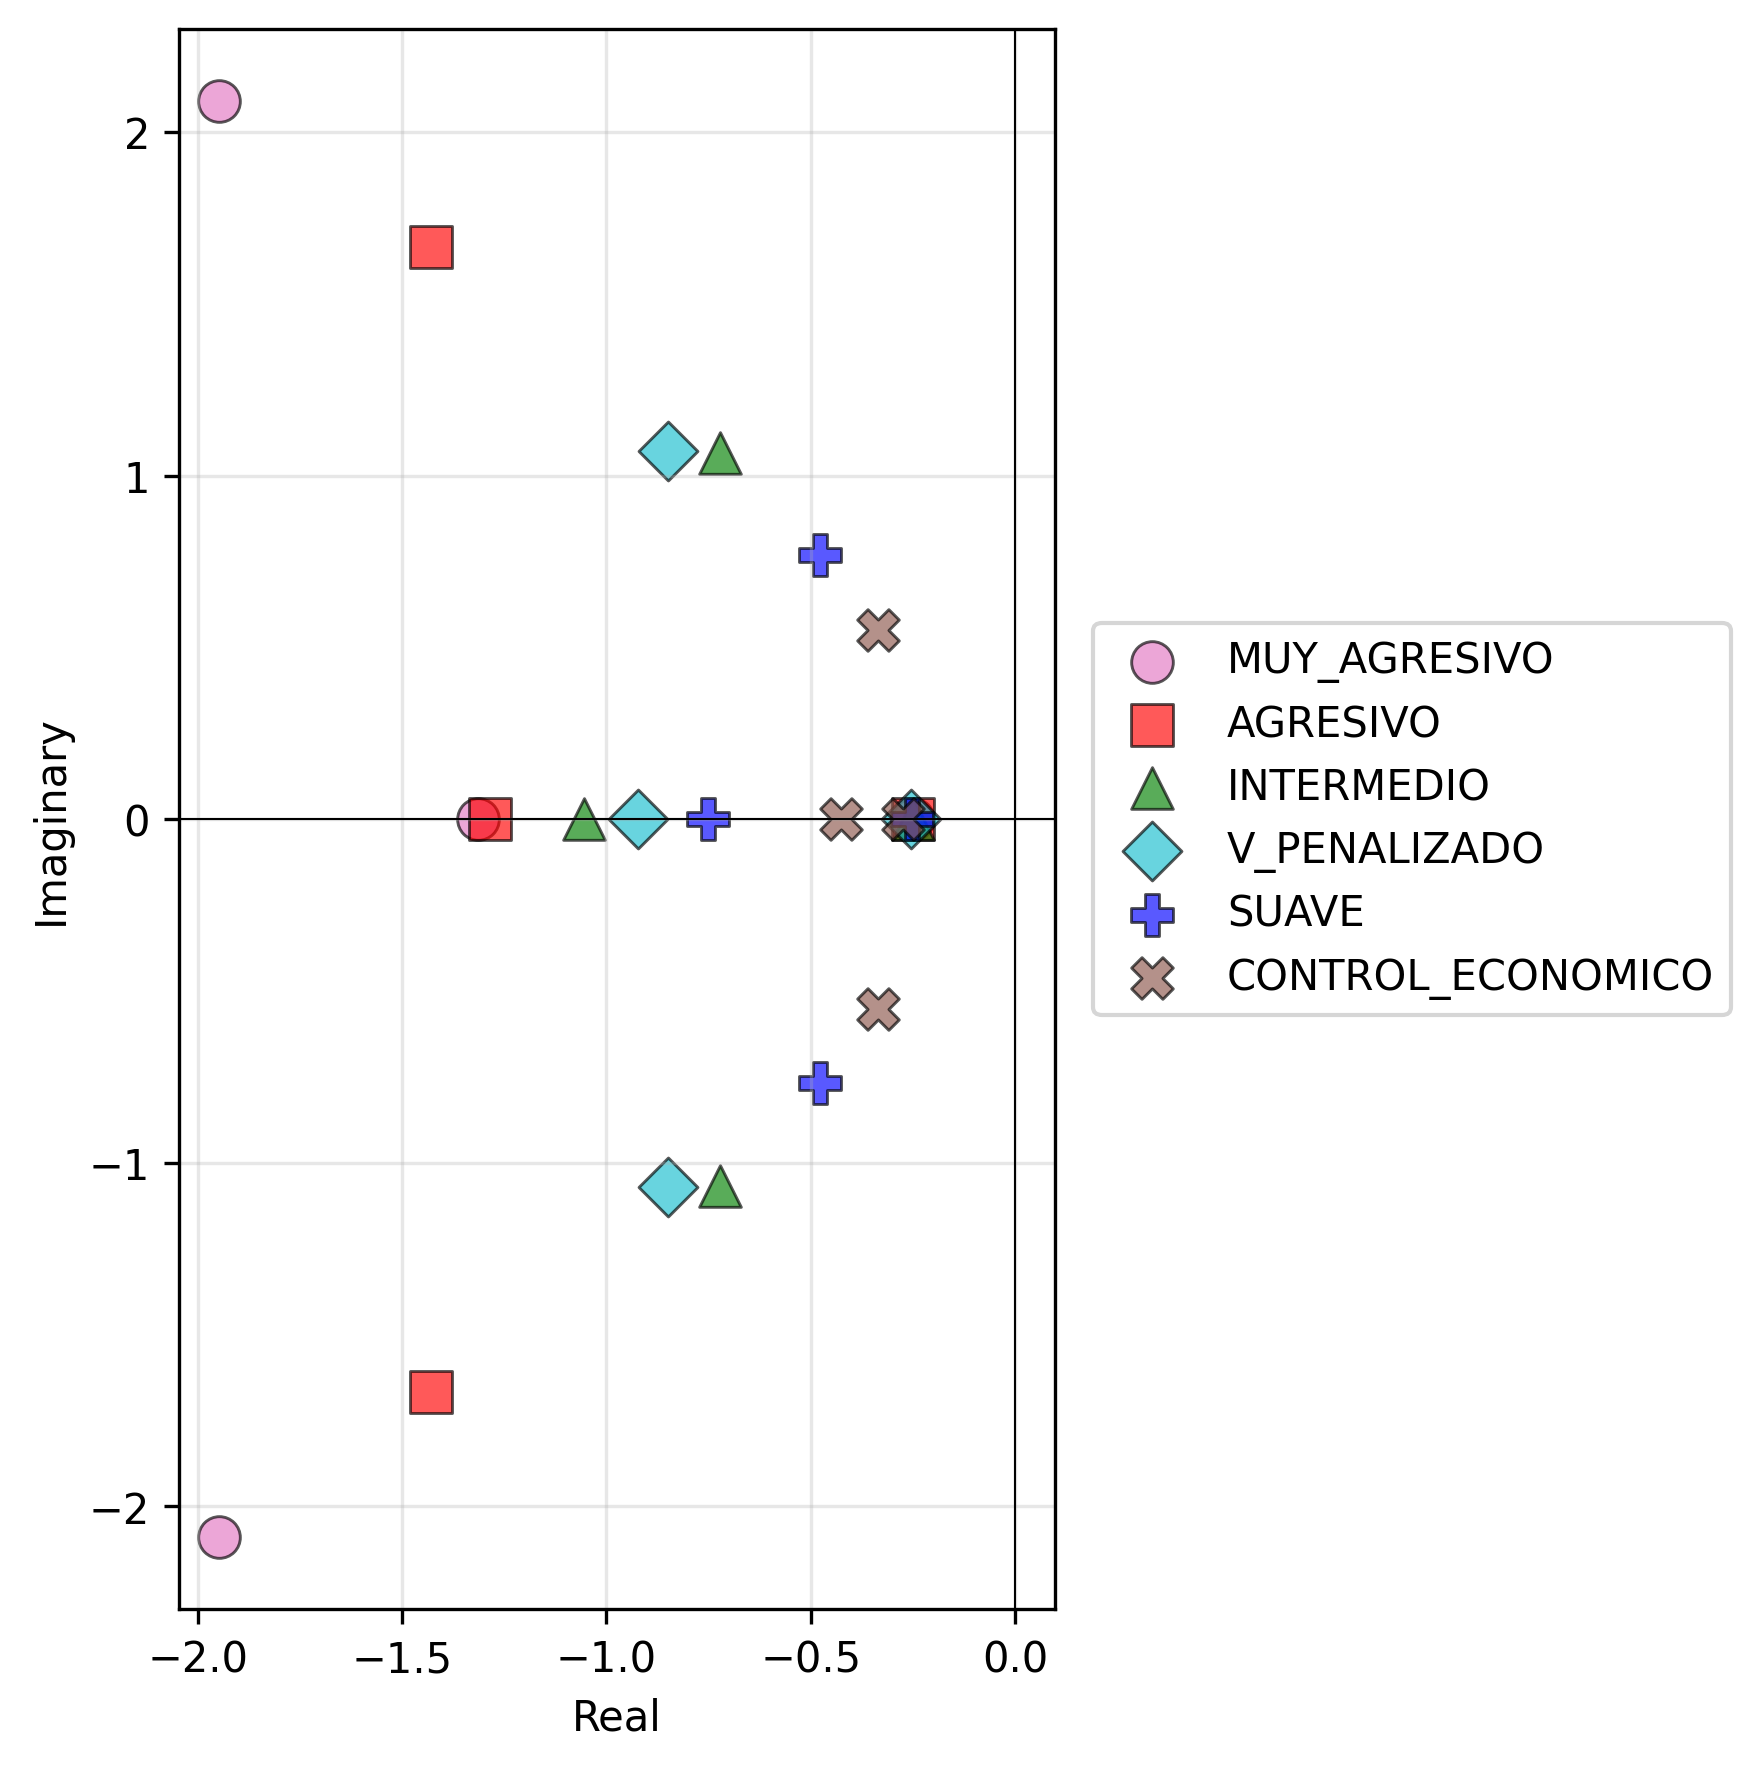
\includegraphics[width=0.88\textwidth]{parteC/lqi/polos.png}
\caption{Polos de lazo cerrado para los controladores LQI evaluados.}
\label{fig:parte-c-polos}
\end{figure}

A medida que el caso se vuelve más agresivo, el par complejo dominante se aleja del eje imaginario y aumenta su parte real negativa. Esto se traduce en una respuesta más rápida. También se observa que uno de los polos reales queda prácticamente fijo cerca de $-0.25$ para varios diseños. Ese polo está asociado a una dinámica del sistema que el cambio de ponderaciones modifica poco en comparación con el par dominante y con el polo ligado al integrador.

\subsection{Comparación entre controladores LQI}

Las Figuras~\ref{fig:parte-c-lqi-seguimiento}, \ref{fig:parte-c-lqi-error}, \ref{fig:parte-c-lqi-control}, \ref{fig:parte-c-lqi-integrador} y~\ref{fig:parte-c-lqi-estados} muestran el desempeño de los seis controladores LQI frente a la misma referencia de rumbo.

\begin{figure}[H]
\centering

\includegraphics[width=0.92\textwidth]{parteC/lqi/seguimiento.png}
\caption{Seguimiento de referencia para los casos LQI.}
\label{fig:parte-c-lqi-seguimiento}
\end{figure}

\begin{figure}[H]
\centering

\includegraphics[width=0.92\textwidth]{parteC/lqi/error.png}
\caption{Error de seguimiento para los casos LQI.}
\label{fig:parte-c-lqi-error}
\end{figure}

\begin{figure}[H]
\centering

\includegraphics[width=0.92\textwidth]{parteC/lqi/control.png}
\caption{Señal de control para los casos LQI.}
\label{fig:parte-c-lqi-control}
\end{figure}

\begin{figure}[H]
\centering

\includegraphics[width=0.92\textwidth]{parteC/lqi/integrador.png}
\caption{Estado del integrador para los casos LQI.}
\label{fig:parte-c-lqi-integrador}
\end{figure}

\begin{figure}[H]
\centering

\includegraphics[width=0.92\textwidth]{parteC/lqi/estados.png}
\caption{Estados del sistema para los casos LQI.}
\label{fig:parte-c-lqi-estados}
\end{figure}

En el seguimiento de referencia se observa que los casos MUY\_AGRESIVO y AGRESIVO son los más rápidos y no presentan sobrepicos importantes respecto de la referencia. Los casos menos agresivos se vuelven progresivamente más lentos a medida que sus polos dominantes se acercan al eje imaginario. En particular, los diseños INTERMEDIO, V\_PENALIZADO, SUAVE y CONTROL\_ECONOMICO muestran sobrepicos que traspasan levemente la referencia luego de los cambios de consigna.

La señal de control permite distinguir mejor los compromisos. MUY\_AGRESIVO y AGRESIVO tienen seguimientos bastante similares, pero el caso MUY\_AGRESIVO requiere un salto considerablemente mayor de control. Por otro lado, el caso INTERMEDIO conserva una respuesta visualmente cercana a los casos agresivos, salvo por un mayor sobrepico, pero reduce de forma marcada el esfuerzo de control. En términos de máximo valor de $\tau_r$, el caso INTERMEDIO requiere menos de la mitad del esfuerzo del caso AGRESIVO y bastante menos que el caso MUY\_AGRESIVO.

\subsection{Comparación con la Parte A}

La comparación entre el controlador por asignación de polos y los controladores LQI se resume en la Tabla~\ref{tab:parte-c-metricas}. Las Figuras~\ref{fig:parte-c-comparacion-seguimiento}, \ref{fig:parte-c-comparacion-error}, \ref{fig:parte-c-comparacion-control}, \ref{fig:parte-c-comparacion-integrador} y~\ref{fig:parte-c-comparacion-estados} muestran las curvas temporales correspondientes.

\begin{table}[H]
\centering
\caption{Comparación de métricas entre la Parte A y los controladores LQI.}
\label{tab:parte-c-metricas}
\scriptsize
\resizebox{\textwidth}{!}{%
\begin{tabular}{lrrrrrrrr}
\toprule
Caso & $\max|\tau_r|$ & RMS $\tau_r$ & $\max|e|$ & IAE & ISE & $e(T_f)$ & $\max|v|$ & $\max|r|$ \\
\midrule
Parte A & 18.599 & 1.908 & 1.981 & 9.271 & 9.829 & 0.00000 & 5.890 & 4.054 \\
MUY\_AGRESIVO & 3.588 & 0.410 & 1.571 & 3.883 & 3.264 & -0.00001 & 2.137 & 1.095 \\
AGRESIVO & 2.647 & 0.340 & 1.571 & 4.301 & 3.766 & -0.00002 & 2.150 & 0.975 \\
INTERMEDIO & 1.314 & 0.222 & 1.571 & 6.013 & 5.416 & -0.00004 & 2.099 & 0.718 \\
V\_PENALIZADO & 1.251 & 0.209 & 1.571 & 6.206 & 5.583 & -0.00029 & 1.988 & 0.674 \\
SUAVE & 0.735 & 0.160 & 1.572 & 8.448 & 7.554 & -0.00011 & 1.906 & 0.526 \\
CONTROL\_ECONOMICO & 0.408 & 0.125 & 1.568 & 12.220 & 11.016 & -0.00369 & 1.608 & 0.361 \\
\bottomrule
\end{tabular}%
}
\end{table}


\begin{figure}[H]
\centering

\includegraphics[width=0.92\textwidth]{parteC/comparacion/seguimiento.png}
\caption{Seguimiento de referencia en la comparación entre Parte A y LQI.}
\label{fig:parte-c-comparacion-seguimiento}
\end{figure}

\begin{figure}[H]
\centering

\includegraphics[width=0.92\textwidth]{parteC/comparacion/error.png}
\caption{Error de seguimiento en la comparación entre Parte A y LQI.}
\label{fig:parte-c-comparacion-error}
\end{figure}

\begin{figure}[H]
\centering

\includegraphics[width=0.92\textwidth]{parteC/comparacion/control.png}
\caption{Señal de control en la comparación entre Parte A y LQI.}
\label{fig:parte-c-comparacion-control}
\end{figure}

\begin{figure}[H]
\centering

\includegraphics[width=0.92\textwidth]{parteC/comparacion/integrador.png}
\caption{Estado del integrador en la comparación entre Parte A y LQI.}
\label{fig:parte-c-comparacion-integrador}
\end{figure}

\begin{figure}[H]
\centering

\includegraphics[width=0.92\textwidth]{parteC/comparacion/estados.png}
\caption{Comparación de estados entre Parte A y los controladores LQI.}
\label{fig:parte-c-comparacion-estados}
\end{figure}

En comparación con la asignación de polos de la Parte A, los controladores LQI reducen de forma importante el esfuerzo de control. Por ejemplo, el caso INTERMEDIO alcanza $\max|\tau_r|=1.314$, frente a $\max|\tau_r|=18.599$ en la Parte A. También disminuye el RMS de la señal de control. Observando únicamente las curvas temporales de rumbo, la Parte A parece converger algo más rápido en algunos cambios de referencia, pero lo hace con sobrepicos y transitorios mucho más agresivos. El caso INTERMEDIO, en cambio, resulta más lento pero menos errático y con una acción de control considerablemente menor. Desde esta perspectiva temporal, el LQI intermedio aparece como una opción más razonable si se busca cuidar el actuador. El costo de esa menor agresividad se analiza en la reconstrucción de trayectorias de la sección siguiente.

\subsection{Reconstrucción de trayectoria para LQI}

Antes de elegir un caso representativo, se comparan las trayectorias reconstruidas de los seis controladores LQI con la trayectoria ideal. El resultado se muestra en la Figura~\ref{fig:parte-c-trayectorias-lqi}.

\begin{figure}[H]
\centering
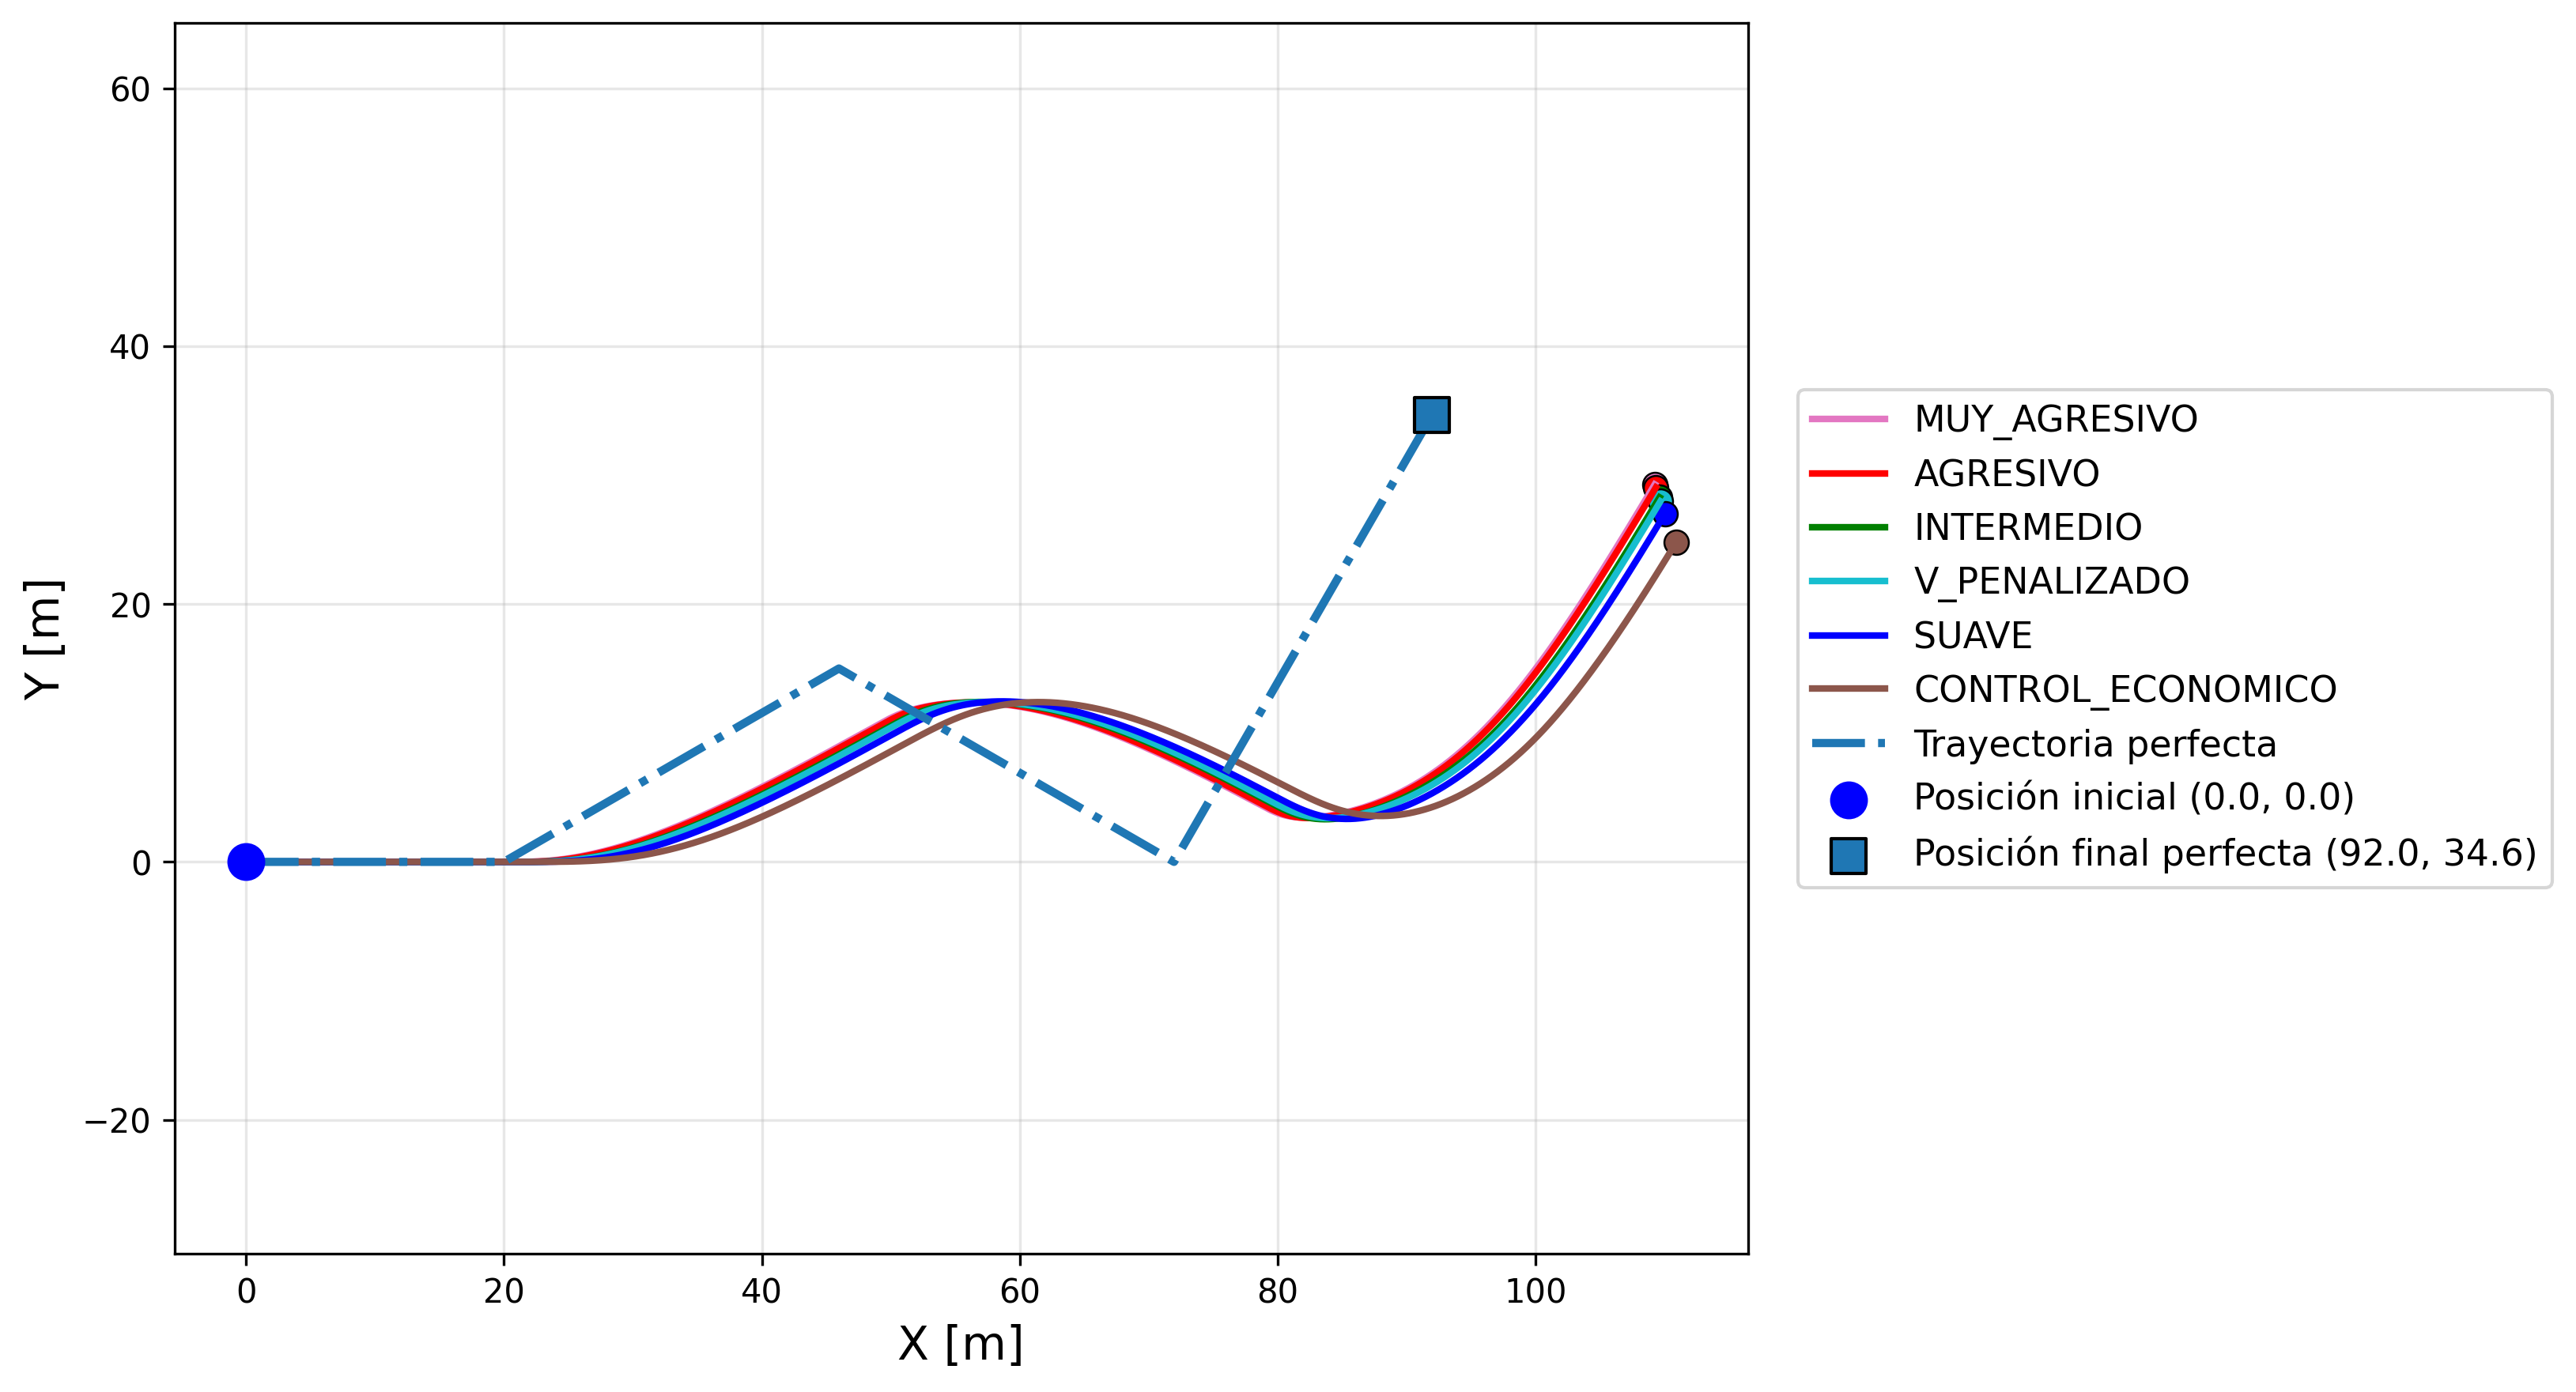
\includegraphics[width=0.86\textwidth]{parteC/lqi/trayectorias_lqi.png}
\caption{Trayectorias reconstruidas para los seis controladores LQI y trayectoria ideal.}
\label{fig:parte-c-trayectorias-lqi}
\end{figure}

\subsection{Trayectorias Parte A y Parte C}

La Tabla~\ref{tab:parte-c-trayectorias} resume las posiciones finales reconstruidas y la distancia respecto de la trayectoria ideal. Allí se observa que la Parte A termina más cerca de la trayectoria perfecta que todos los casos LQI. Esto se debe a que su respuesta de rumbo es más agresiva y rápida, lo que ayuda a respetar más fielmente los cambios de dirección esperados en el plano $X,Y$.

\begin{table}[H]
\centering
\caption{Posición final reconstruida y distancia a la trayectoria ideal.}
\label{tab:parte-c-trayectorias}
\begin{tabular}{lrrr}
\toprule
Caso & $X_f$ [m] & $Y_f$ [m] & Distancia a ideal [m] \\
\midrule
Perfecta & 91.96 & 34.64 & 0.00 \\
Parte A & 97.40 & 38.14 & 6.47 \\
MUY\_AGRESIVO & 109.24 & 29.28 & 18.09 \\
AGRESIVO & 109.33 & 29.05 & 18.25 \\
INTERMEDIO & 109.61 & 28.27 & 18.77 \\
V\_PENALIZADO & 109.68 & 27.97 & 18.93 \\
SUAVE & 110.04 & 27.02 & 19.62 \\
CONTROL\_ECONOMICO & 110.92 & 24.82 & 21.35 \\
\bottomrule
\end{tabular}
\end{table}


Entre los controladores LQI, la mayoría de las trayectorias termina relativamente cerca una de otra; las diferencias más claras aparecen en los diseños más lentos, especialmente CONTROL\_ECONOMICO. El caso INTERMEDIO queda dentro del grupo principal de trayectorias LQI: no es el más cercano a la trayectoria ideal, pero su posición final es similar a la de los casos más agresivos. Al mismo tiempo, requiere mucho menos esfuerzo de control que MUY\_AGRESIVO y AGRESIVO. Por ese motivo se elige como controlador representativo de la Parte C.

\begin{figure}[H]
\centering
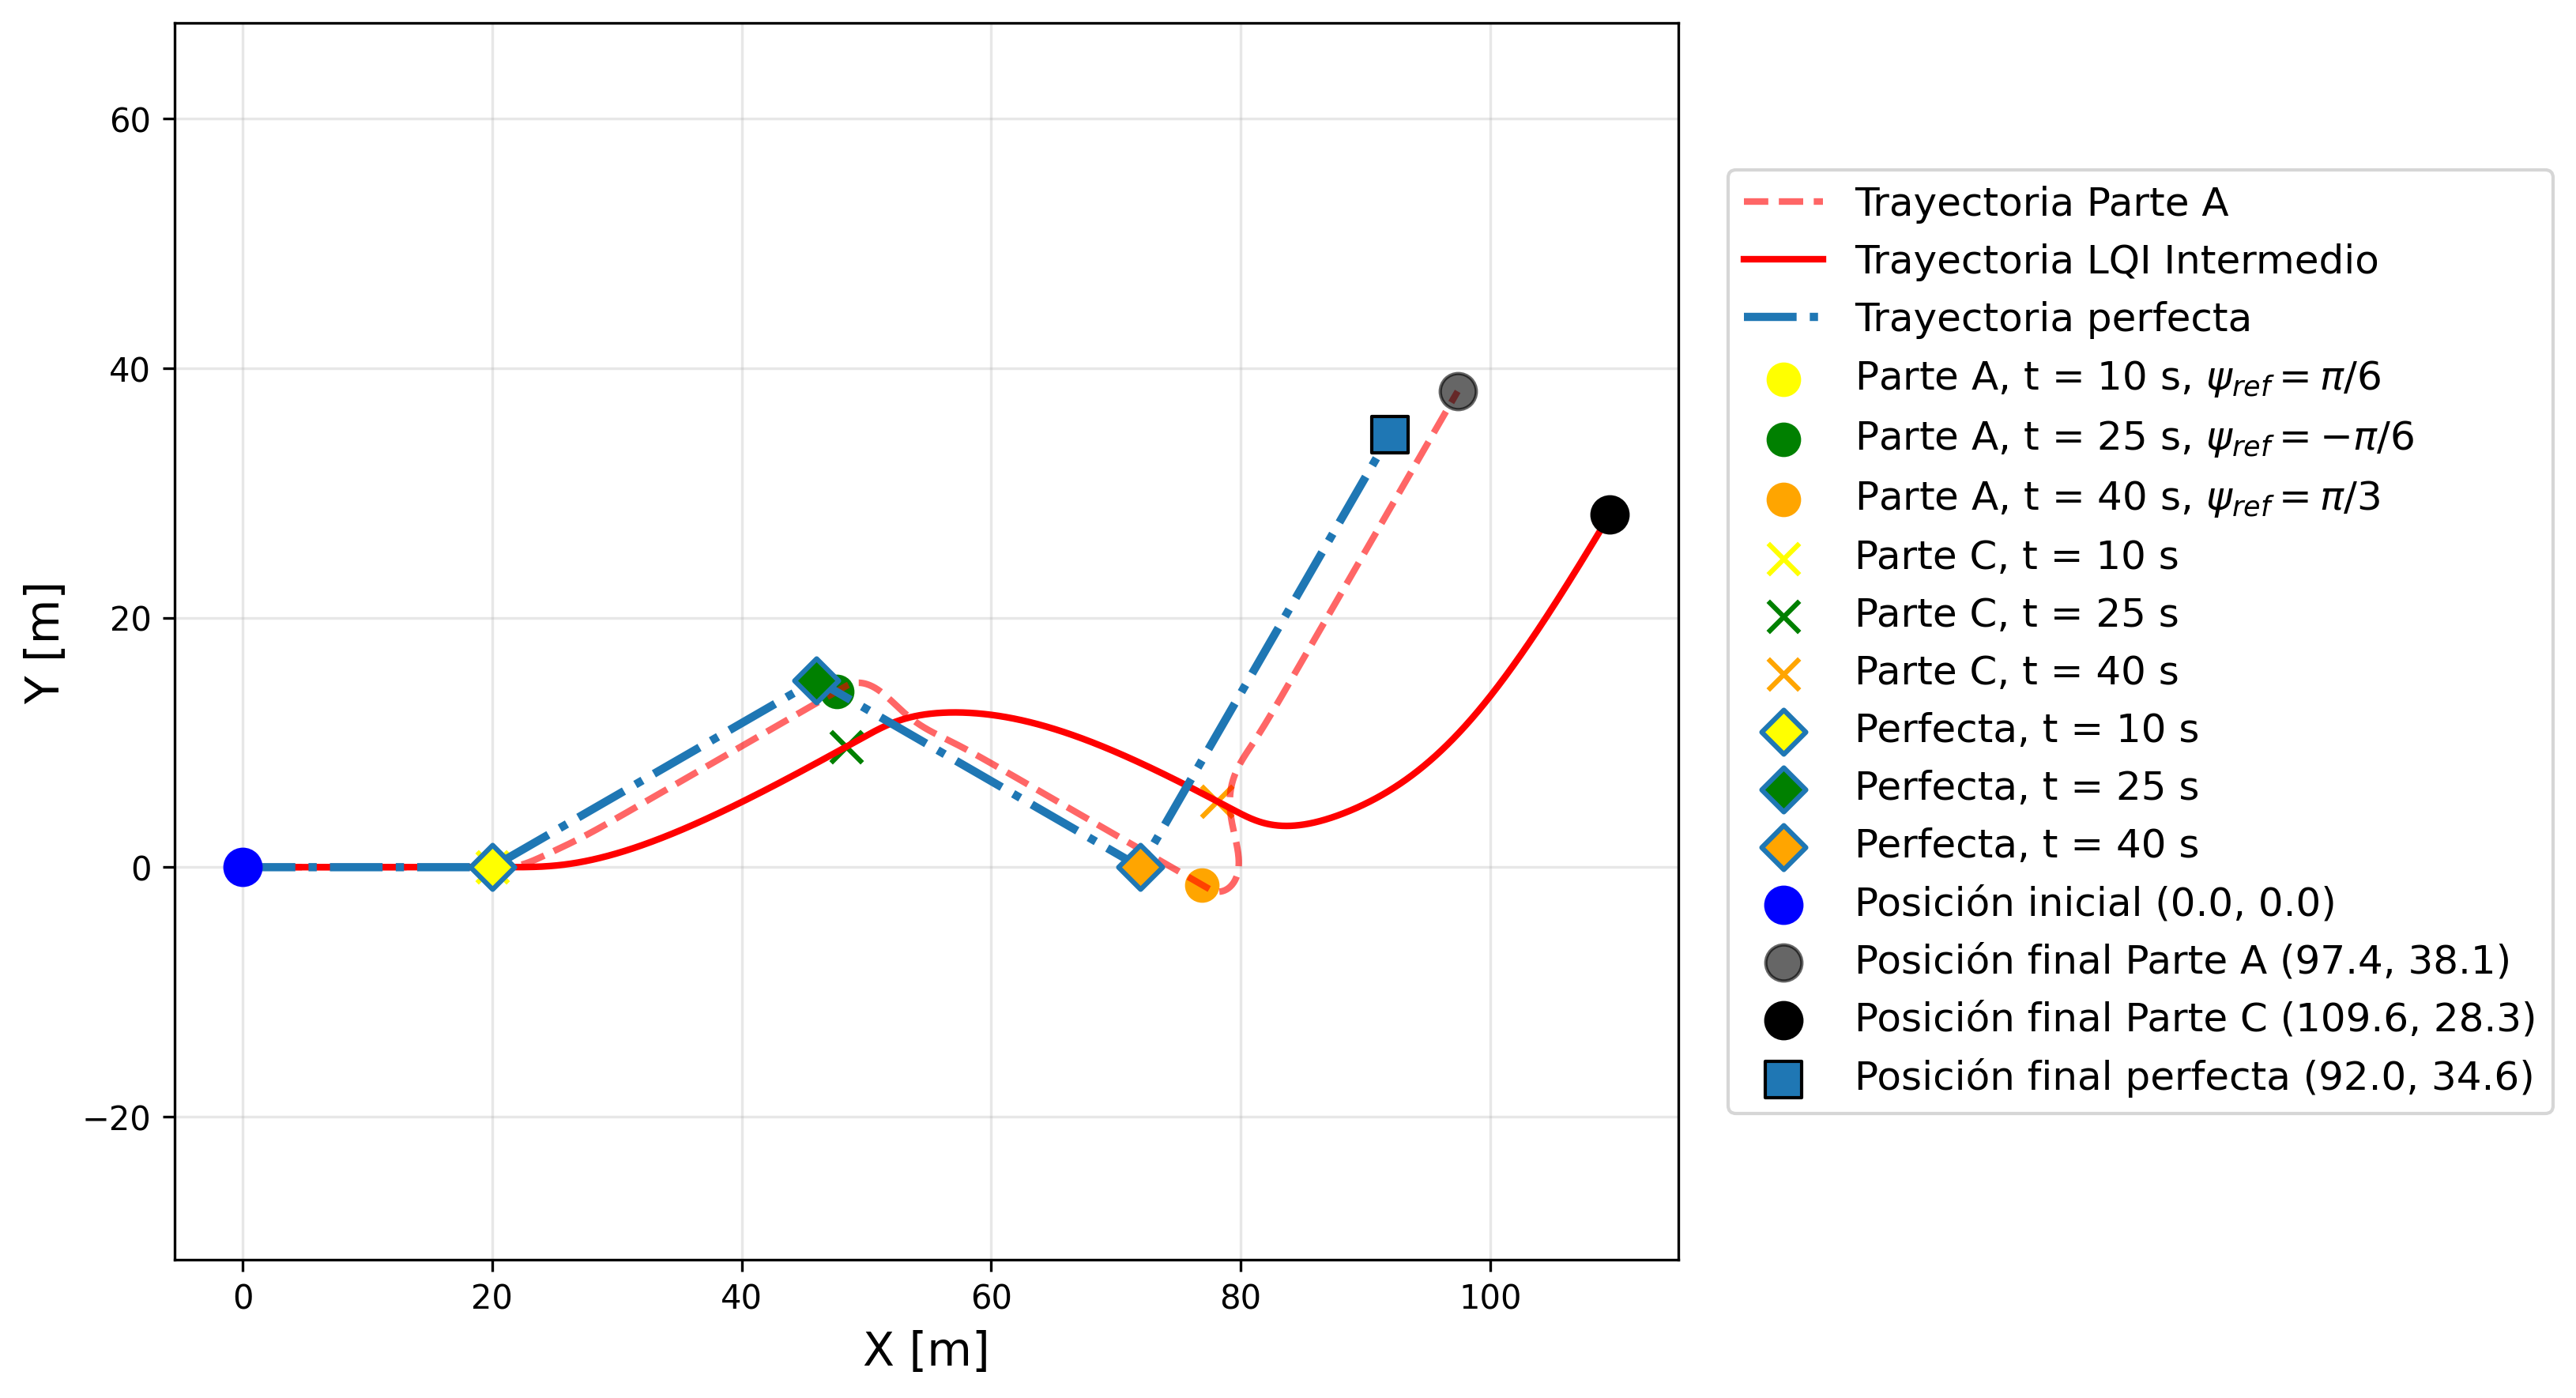
\includegraphics[width=0.88\textwidth]{parteC/comparacion/trayectoria_parteA_vs_lqi_intermedio.png}
\caption{Comparación de trayectorias entre Parte A, LQI intermedio y trayectoria ideal.}
\label{fig:parte-c-trayectoria-comparacion}
\end{figure}

La Figura~\ref{fig:parte-c-trayectoria-comparacion} muestra la diferencia entre ambas alternativas. El LQI intermedio reduce fuertemente el esfuerzo de control, pero su menor rapidez de convergencia hace que la embarcación avance durante más tiempo con un rumbo intermedio entre la referencia anterior y la nueva. Esa lentitud acumulada se transforma en una diferencia importante de posición final. En cambio, la agresividad de la Parte A permite corregir el rumbo más cerca de los instantes de cambio de referencia y por eso respeta mejor la trayectoria ideal. La pregunta de diseño pasa entonces a ser física: si el actuador y la embarcación soportan esa agresividad, la Parte A reproduce mejor la trayectoria; si no, el LQI intermedio es una alternativa más realista y suave.

\subsection{Ventajas y desventajas de asignación de polos y LQI}

La asignación de polos tiene como ventaja principal que permite imponer de forma directa la dinámica deseada del sistema aumentado. Es un método claro para fijar la velocidad de respuesta y garantizar estabilidad si el sistema es controlable. En este trabajo esa rapidez también favorece la reconstrucción de trayectoria, ya que el rumbo se corrige cerca de los instantes en que cambia la referencia. Sin embargo, el método no optimiza el esfuerzo de control y puede producir señales de control muy elevadas, como se observa en la Parte A.

El LQI, en cambio, permite incorporar compromisos de diseño mediante $Q_a$ y $R$. Esto hace posible reducir el esfuerzo de control y ajustar la respuesta de manera más gradual. Su desventaja es que la elección de pesos no es única y requiere un proceso de diseño iterativo: modificar $Q_a$ y $R$ cambia simultáneamente seguimiento, esfuerzo, polos y trayectoria. Además, como el costo LQI se formula sobre el rumbo y los estados aumentados, no garantiza por sí solo que la trayectoria en $X,Y$ sea la más cercana a la ideal. En este problema, LQI resulta conveniente cuando se busca cuidar la señal de control, mientras que la asignación de polos es útil si se prioriza una respuesta rápida y directa.

\FloatBarrier


\section{Conclusiones}

\pendiente{Redactar una conclusión global: resumir si el controlador por polos cumple el seguimiento, por qué LQI reduce el esfuerzo de control, qué compromiso se eligió y cuáles serían los pasos siguientes si se quisiera controlar posición en el plano.}

\end{document}
